\section{Generalized Gamma Algebra for Fat Tails}

\begin{frame}{High-level Idea}
    \begin{figure}
        \centering
        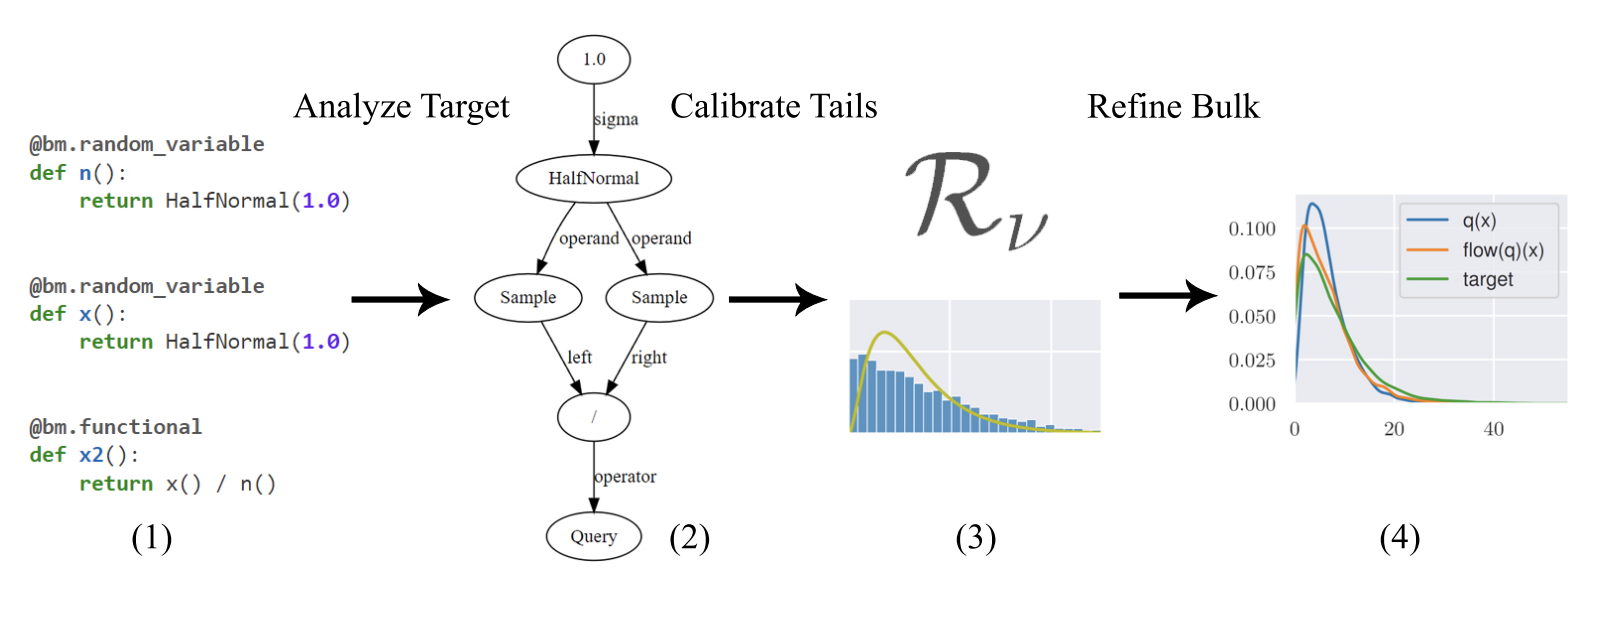
\includegraphics[width=1\textwidth]{Figures/gga/schematic.png}
    \end{figure}
\end{frame}

\begin{frame}{Generalized gamma tail parameterization}
    \begin{definition}
        Let $\nu \in \mathbb{R}$, $\sigma > 0$, and $\rho \in \mathbb{R} \backslash \{0\}$ be such that $(\nu+1)/ \rho > 0$.
        A non-negative random variable $X$ is \emph{generalized Gamma distributed} with parameters $\nu,\sigma,\rho$ if it has Lebesgue density
        \begin{equation}
        \label{eq:GenGammaDensity}
        p_{\nu,\sigma,\rho}(x) = c_{\nu,\sigma,\rho} x^\nu e^{-\sigma x^\rho},\qquad x > 0,
        \end{equation}
        where $c_{\nu,\sigma,\rho} = \rho \sigma^{(\nu+1)/\rho} / \Gamma((\nu+1)/\rho)$ is the normalizing constant. %The generalized Gamma density incorporates many other well-known densities, including that of the Gamma distribution ($\rho = 1$), and the Frechet/Weibull distribution ($\nu = \rho - 1$). 
    \end{definition}
\end{frame}

\begin{subframe}{Static analysis in PPL}
    \begin{algorithm}[H]
    	\caption{Pseudocode for a GGA tails static analysis pass}\label{alg:bfs_typecheck}
    	\KwData{Abstract syntax tree for a PPL program}
    	\KwResult{GGA parameter estimates for all random variables}
    	frontier $\gets$ [rv : Parents(rv) = $\emptyset$]\;
    	GGAs $\gets \{\}$\;
    	\While{\text{frontier} $\neq \emptyset$}{
    		next $\gets$ frontier.popLeft()\;
    		GGAs[next] $\gets$ computeGGA(next.op, next.parent)\;
    		frontier $\gets$ frontier + next.children()\;
    	}
    	\Return{GGAs}
    \end{algorithm}
\end{subframe}

\begin{frame}{Prior work \parencite{resnick2007heavy}: closure under addition}
    \begin{align*}
        &  (\nu_{1},\sigma_{1},\rho_{1})\oplus(\nu_{2},\sigma_{2},\rho_{2}) \\
        & \equiv \begin{cases}
            \max\{(\nu_{1},\sigma_{1},\rho_{1}),(\nu_{2},\sigma_{2},\rho_{2})\} & \text{ if }\rho_{1}\neq\rho_{2}\text{ or }\rho_{1},\rho_{2}<1\\
            \left(\nu_{1}+\nu_{2}+1,\min\{\sigma_{1},\sigma_{2}\},1\right) & \text{ if }\rho_{1}=\rho_{2}=1\\
            (\nu_{1}+\nu_{2}+\frac{2-\rho}{2},(\sigma_{1}^{-\frac{1}{\rho-1}}+\sigma_{2}^{-\frac{1}{\rho-1}})^{1-\rho},\rho) & \text{ if }\rho=\rho_{1}=\rho_{2}>1.
        \end{cases}
    \end{align*}
\end{frame}

\begin{frame}{New: closure under multiplication\footnote{\fullcite{gga}}}
    \begin{align*}
        & (\nu_{1},\sigma_{1},\rho_{1})\otimes(\nu_{2},\sigma_{2},\rho_{2}) \\
        &\qquad \equiv\begin{cases}
        \left(\frac{1}{\mu}\left(\frac{\nu_{1}}{|\rho_{1}|}+\frac{\nu_{2}}{|\rho_{2}|}+\frac{1}{2}\right),\sigma,-\frac{1}{\mu}\right) & \text{ if }\rho_{1},\rho_{2}<0\\
        \left(\frac{1}{\mu}\left(\frac{\nu_{1}}{\rho_{1}}+\frac{\nu_{2}}{\rho_{2}}-\frac{1}{2}\right),\sigma,\frac{1}{\mu}\right) & \text{ if }\rho_{1},\rho_{2}>0\\
        \mathcal{R}_{|\nu_1|} & \mbox{ if }\rho_{1}\leq0,\rho_{2}>0 \\
        \mathcal{R}_{\min\{|\nu_1|,|\nu_2|\}} & \mbox{ if }\rho_{1}=0,\rho_{2}=0
        \end{cases} \\
        &\text{where }\mu=\frac{1}{|\rho_{1}|}+\frac{1}{|\rho_{2}|}=\frac{|\rho_{1}|+|\rho_{2}|}{|\rho_{1}\rho_{2}|}, \sigma=\mu(\sigma_{1}|\rho_{1}|)^{\frac{1}{\mu|\rho_{1}|}}(\sigma_{2}|\rho_{2}|)^{\frac{1}{\mu|\rho_{2}|}}.
    \end{align*}
\end{frame}

\begin{frame}{New: closure under Lipschitz maps, bulk correction}
    \begin{align*}
        & f(X_1,\dots,X_n) \equiv L \max\{X_1,\dots,X_n\}
    \end{align*}
    \begin{figure}
        \centering
        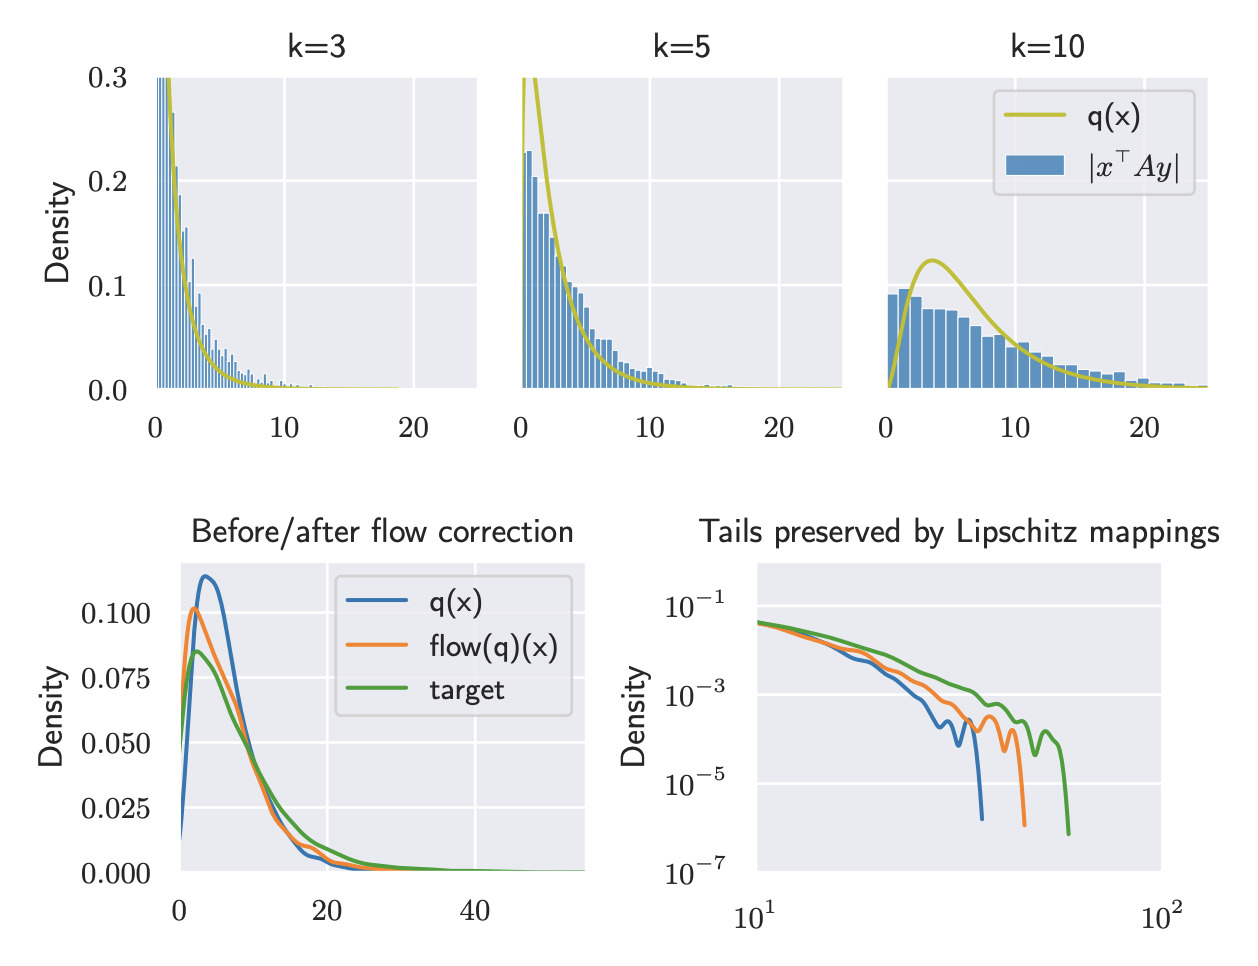
\includegraphics[width=0.7\textwidth]{Figures/gga/flow-correction.png}
    \end{figure}
\end{frame}

\begin{frame}{Results: variational inference}
    \begin{figure}
        \centering
        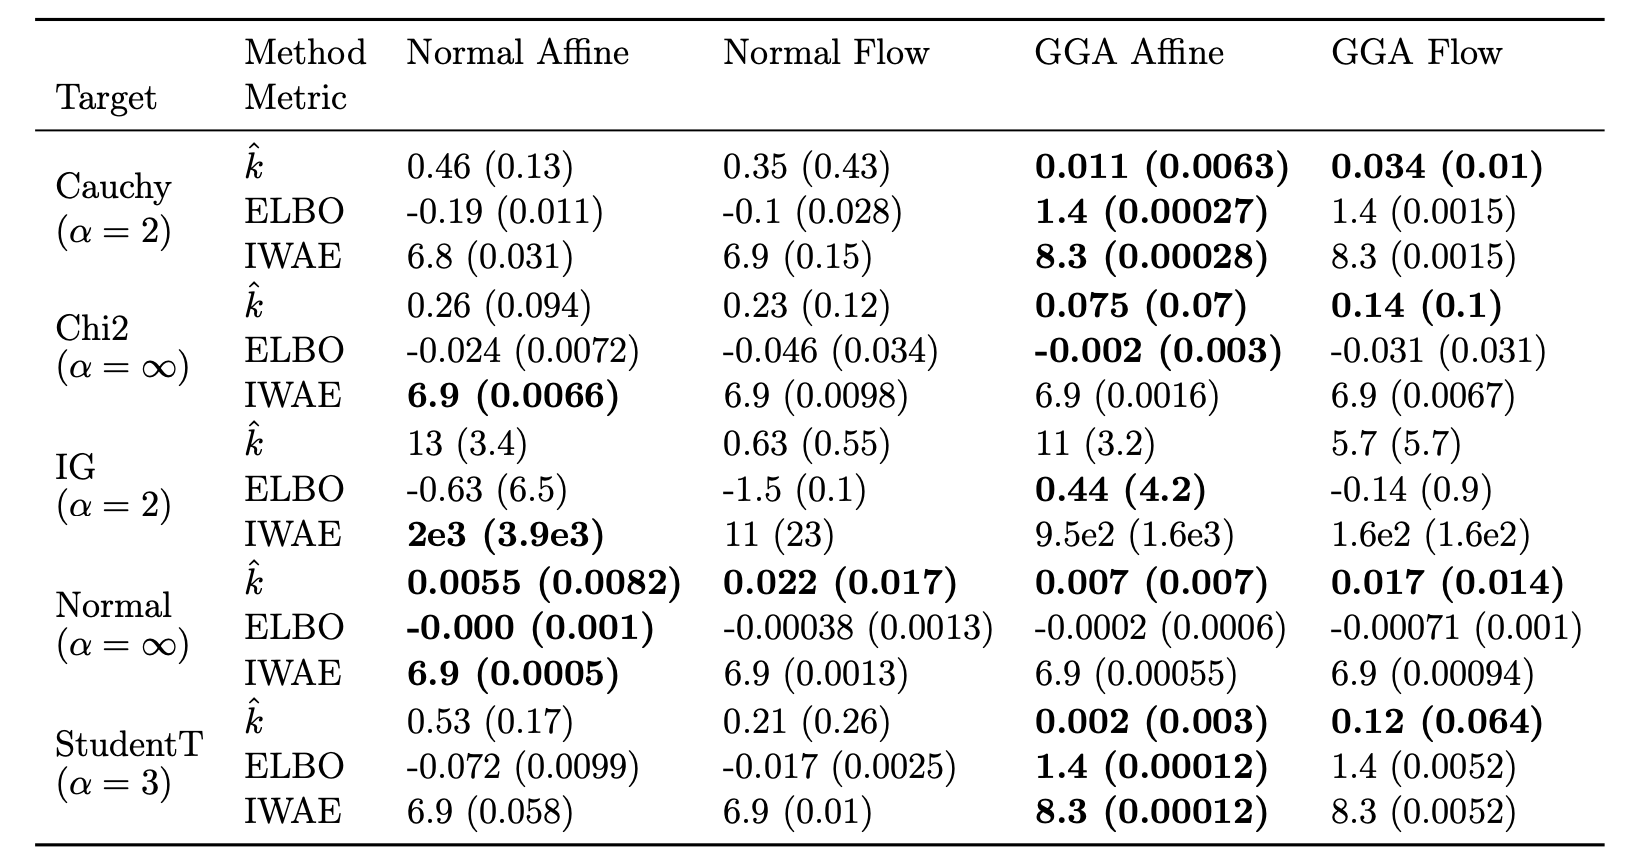
\includegraphics[width=\textwidth]{Figures/gga/vi.png}
    \end{figure}
\end{frame}

\begin{frame}{Results: density estimation}
    \begin{figure}
        \centering
        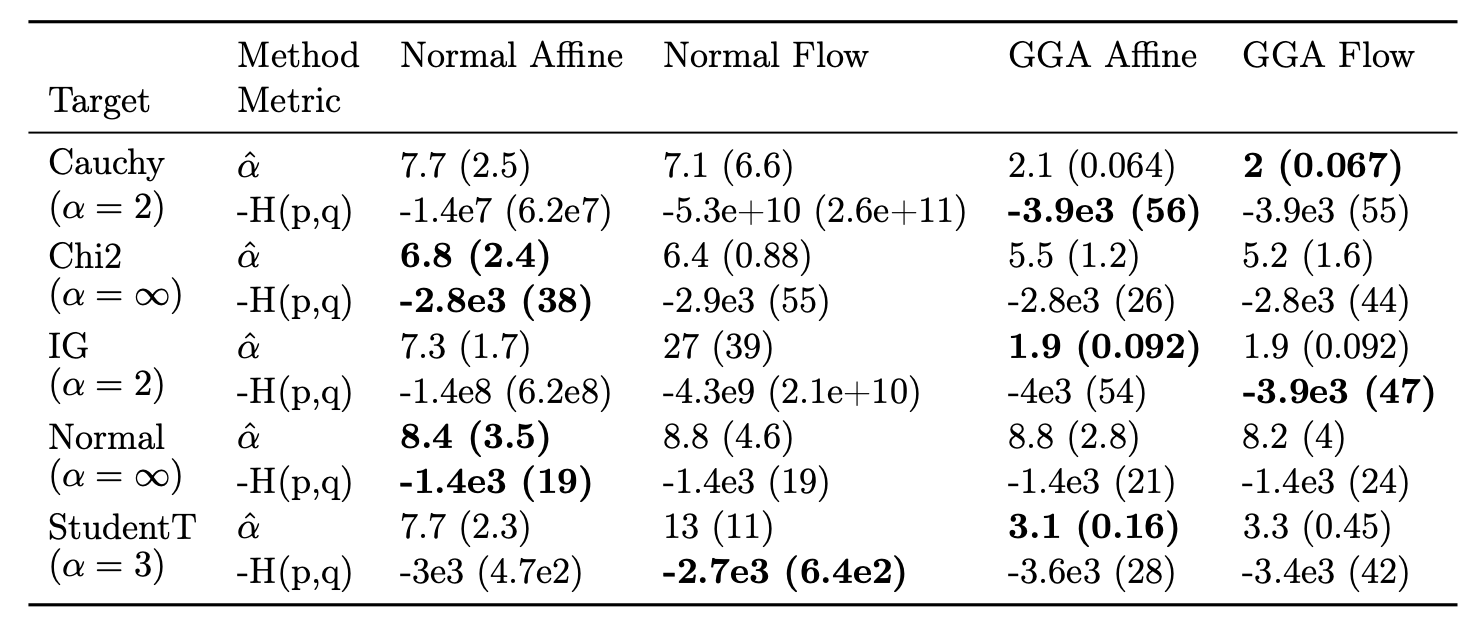
\includegraphics[width=\textwidth]{Figures/gga/de.png}
    \end{figure}
\end{frame}